\documentclass{article}
\usepackage{graphicx} % Required for inserting images
\usepackage{hyperref}
\usepackage{caption} % For custom captions
\usepackage{amsmath}
\usepackage{animate}
\usepackage{multicol}
\usepackage{subcaption}

\title{Theoretical Mechanics: Week Homework 7}
\author{Ekaterina Mozhegova}
\date{March 13, 2024}

\begin{document}

\maketitle

\section{Link}
\href{https://github.com/illusoryTwin/Theoretical_mechanics/tree/master/hw7}{Link to the github repository containing all the materials}

\section{Task 1}

\subsection{Task Description}

A step ladder $ABC$, hinged at $B$, rests on a smooth horizontal floor, as shown on the figure. $AB=BC=2l$.

The centres of gravity are at the midpoints $D$ and $E$ of the rods. The radius of gyration of each part of the ladder about the axis passing through the center of gravity is $p$.

The distance between $B$ and the floor is $h$. At the certain moment the ladder collapses due to the rupture of a ling $FG$ between the two halves of the ladder. Neglecting the effect of friction in the hinge, determine:
\begin{enumerate}
  \item the velocity $v_1$ of the point $B$ at the moment, when it hits the floor;
  \item the velocity $v_2$ of point $B$ at the moment, when it is at a distance $\dfrac{1}{2}h$ from the floor.
\end{enumerate}

\includegraphics*[scale=0.5]{task_scheme/hw7_task1.png}{\centering}
\subsection{Task Explanation}

\textbf{Research object:} A system of 2 rods: rod 1 and rod 2\\
\textbf{Motion:} rod 1 - rotational and plane motions, rod 2 - rotational and plane motions\\
\textbf{Force analysis:} $G_1 = m_1 g$, $G_2 = m_2 g$\\

\begin{center}
  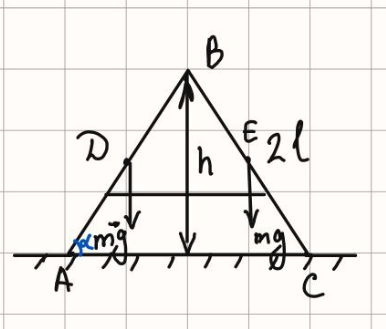
\includegraphics[scale=0.35]{task_scheme/task1_forces.png}
\end{center}


\textbf{Solution:}

\[T = A \text{, where } T = \sum T_i, A = \sum A_i\]
\[T = T_1 + T_2 = 2T_1 \text{(due to the system's symmetry)}\] 
\[T_1 = \dfrac{m v_d^2}{2} + \dfrac{J \omega^2}{2} = \dfrac{m v_d^2}{2} + \dfrac{m \rho^2 \omega^2}{2}\] (plane motion  and rotational motion)
\[v_d^2 = \dot y_d^2 + \dot x_d^2\]



\begin{align*}
    y_d &= l \sin(\alpha) & \dot{y}_d &= l \dot{\alpha} \cos(\alpha) \\
    x_d &= l \cos(\alpha) & \dot{x}_d &= -l \dot{\alpha} \sin(\alpha)
\end{align*}


\[ \dot \alpha = \omega = \dot \alpha = \dfrac{v_b}{2l \cos \alpha}\]

\[V_d^2 = (l \cos(\alpha) \dot{\alpha})^2 + (-l \sin(\alpha) \dot{\alpha})^2 = l^2 (\dot{\alpha})^2 = l \omega^2\]

\[V_d^2 = l^2 \omega^2 = l^2 \cdot \frac{v_b^2}{4l^2 \cos^2(\alpha)}\]

\[T_\text{rot} = \dfrac{J \omega^2}{2} = \dfrac{m \rho^2 \omega^2}{2} = \dfrac{m \rho^2}{2} \dfrac{V_b^2}{4l^2 \cos(\alpha)^2}\]

\[T_1 = T + T_{\text{rot}} = \frac{mV_d^2}{2} + \frac{J \omega^2}{2} = \frac{m V_b^2}{2 \cdot 4 \cos^2(\alpha)} + \frac{m \rho^2 V_b^2}{2 \cdot 4l^2 \cos^2(\alpha)}\]

\[T_\text{tot} = 2T_1 = 2 (\frac{m V_b^2}{2 \cdot 4 \cos^2(\alpha)} + \frac{m \rho^2 V_b^2}{2 \cdot 4l^2 \cos^2(\alpha)}) = \frac{m V_b^2}{4 \cos^2(\alpha)} + \frac{m \rho^2 V_b^2}{4l^2 \cos^2(\alpha)}\]

\textbf{Work:}

2 gravitational forces do the work ($G_1$ of a rod 1 and $G_2$ of a rod 2).

Due to the symmetry:

\[A_\text{tot} = 2A_G = 2 mg \Delta h = 2mg ( \frac{h}{2} - l \sin(\alpha))\]
 
\begin{center}
  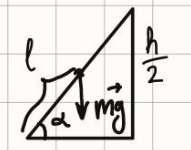
\includegraphics[scale=0.35]{task_scheme/task1_scheme.png}
\end{center}


\begin{enumerate}
  \item When B hits the floor, $\alpha = 0$, so $A_\text{tot} = 2 m g \frac{h}{2} = mgh$
    \begin{center}
      For $\alpha = 0$ we have: $\cos(\alpha) = 1$, $\sin(\alpha) = 0$.
    \end{center}
    \[ \frac{m V_b^2}{4 \cos^2(\alpha)} + \frac{m \rho^2 V_b^2}{4l^2 \cos^2(\alpha)} = mgh\]
    \[ \frac{m V_b^2}{4 \cdot 1} (1 + \frac{\rho^2}{l^2}) = mgh\]
    \[ \frac{V_b^2}{4} (\frac{l^2 + \rho^2}{l^2}) = gh\]
    \[ V_b = \sqrt{\dfrac{4l^2gh}{l^2 + \rho^2}} = 2l \sqrt{\dfrac{gh}{l^2 + \rho^2}}\]
    \[ \text{So, } V_b = 2l \sqrt{\dfrac{gh}{l^2 + \rho^2}}\]


  \item When B  is at the distance $ \frac{1}{2} h$ from the floor. 
    \[\sin(\alpha) = \dfrac{\frac{h}{2}}{2l} = \dfrac{h}{4l}\]
    \[\text{Thus, } \cos(\alpha)^2 = 1 - \sin(\alpha)^2 = \dfrac{16l^2 - h^2}{16l^2}\]
    \[ \frac{m V_b^2}{4 \cdot \dfrac{16l^2 - h^2}{16l^2}} (\dfrac{\rho^2 + l^2}{l^2}) = 2mg(\frac{h}{2} - l \sin(\alpha))\]
    \[ \frac{m V_b^2}{\dfrac{16l^2 - h^2}{4l^2}} (\dfrac{\rho^2 + l^2}{l^2}) = 2mg(\frac{h}{2} - l \frac{h}{4l})\]
    \[ \frac{4 mV_b^2 (l^2+\rho^2)}{16l^2 - h^2} = \dfrac{mgh}{2}\]
    \[ \frac{4 V_b^2 (l^2+\rho^2)}{16l^2 - h^2} = \dfrac{gh}{2}\]
    \[ V_b = \sqrt{\dfrac{gh(16l^2-h^2)}{2 \cdot 4(l^2 + \rho^2)}} = \dfrac{1}{2} \sqrt{\dfrac{gh(16l^2 - h^2)}{2(l^2 + \rho^2)}}\]
    \[ \text{So, } V_b = \dfrac{1}{2} \sqrt{\dfrac{gh(16l^2 - h^2)}{2(l^2 + \rho^2)}}\]
\end{enumerate}

\textbf{Answer:}
\begin{enumerate}
  \item \[V_b = 2l \sqrt{\dfrac{gh}{l^2 + \rho^2}}\]
  \item \[V_b = \dfrac{1}{2} \sqrt{\dfrac{gh(16l^2 - h^2)}{2(l^2 + \rho^2)}}\]
\end{enumerate}

\section{Task 2}

\subsection{Task Description}

You should solve this problem using:
\begin{enumerate}
  \item \textbf{Newton-Euler} method;
  \item Model-oriented design applications (\textit{SimInTech}, or MATLAB Simulink).
\end{enumerate}
\textbf{Tasks}
\begin{enumerate}
  \item To derive a differential equation of the motion, using \textbf{Newton-Euler} approach.
  \item To create plots $x(t),\ \phi(t), \dot{x}(t), \dot{\phi}(t)$. 
  \item To make a simulation of this system. Show velocities and accelerations for $1,\ 2$ bodies (coding approach).
\end{enumerate}
\textbf{Artifacts}
\begin{enumerate}
  \item Report in \textit{.pdf} or in \textit{.md}.
  \item For \textbf{Newton-Euler} method --- code, GIFs, plots.
  \item For \textbf{SimInTech} --- \textit{.prt}, for \textbf{Simulink} --- \textit{.slx} file which contains a description of the system, GIFs, plots.
\end{enumerate}


\includegraphics*[scale=0.5]{task_scheme/hw8_task2.png}{\centering}
   
\subsection{Task Explanation}

\textbf{Research object:} A system of 2 bodies: cart and pole\\
\textbf{Motion:} A cart - plane motion, pole - rotational motion\\
\textbf{Force analysis:} $G_1 = m_1 g$, $G_2 = m_2 g, T, N,  m_2 \ddot x \text{ - inertial force}$\\
\textbf{Solution:}

(1) \text{Cart:}
\[
\begin{cases}
  \text{X:} & -T_x - m_1 \ddot x = 0 \\
  \text{Y:} & N = G_1 + T_y
\end{cases}
\]

(2) \text{Pole:}
\[
\begin{cases}
  \text{X:} & T_x = m_2 a_{2x} + m_2 \ddot x\\
  \text{Y:} & T_y - G_2 = m_2 a_{2y}
\end{cases}
\]


% \begin{equation}\label{eq:example}
%   J \epsilon = J \ddot \phi = -G_2 l \cos(\frac{\pi}{2} - \phi) - m_2 \ddot x l \cos(\phi)
% \end{equation}


\[J \epsilon = J \ddot \phi = -G_2 l \cos(\frac{\pi}{2} - \phi) - m_2 \ddot x l \cos(\phi)\]

Acceleration of the pole $\vec a_2$ is the sum of tangential and centripetal acceleration:

\[\vec{a}_2 = \vec{\dot{\phi}}^2 \cdot l + \vec{\ddot{\phi}} \cdot l\]

Projections of $vec{a}_2$ are the following:
\[a_{2x} = -\dot{\phi}^2 l \sin(\phi) + \ddot{\phi} l \cos(\phi)\]
\[a_{2y} = \dot{\phi}^2 l \cos(\phi) + \ddot{\phi} l \sin(\phi)\]

So, 

\[
\begin{cases}
  -T_x - m_1 \ddot x = 0 \\
  N = G_1 + T_y\\
  T_x = m_2 (-\dot{\phi}^2 l \sin(\phi) + \ddot{\phi} l \cos(\phi)) + m_2 \ddot x\\
  T_y - G_2 = m_2 (\dot{\phi}^2 l \cos(\phi) + \ddot{\phi} l \sin(\phi))\\
  J \ddot \phi = -G_2 l \cos(\frac{\pi}{2} - \phi) - m_2 \ddot x l \cos(\phi)
\end{cases}
\]

Or:

\[
\begin{cases}
  -T_x - m_1 \ddot x = 0 \\
  N = m_1g + T_y\\
  T_x = m_2 (-\dot{\phi}^2 l \sin(\phi) + \ddot{\phi} l \cos(\phi)) + m_2 \ddot x\\
  T_y - m_2g = m_2 (\dot{\phi}^2 l \cos(\phi) + \ddot{\phi} l \sin(\phi))\\
  J \ddot \phi = -m_2g l \cos(\frac{\pi}{2} - \phi) - m_2 \ddot x l \cos(\phi)
\end{cases}
\]

Solving the system computationally will provide us with the results below.


\subsection{Plots}

\begin{center}
  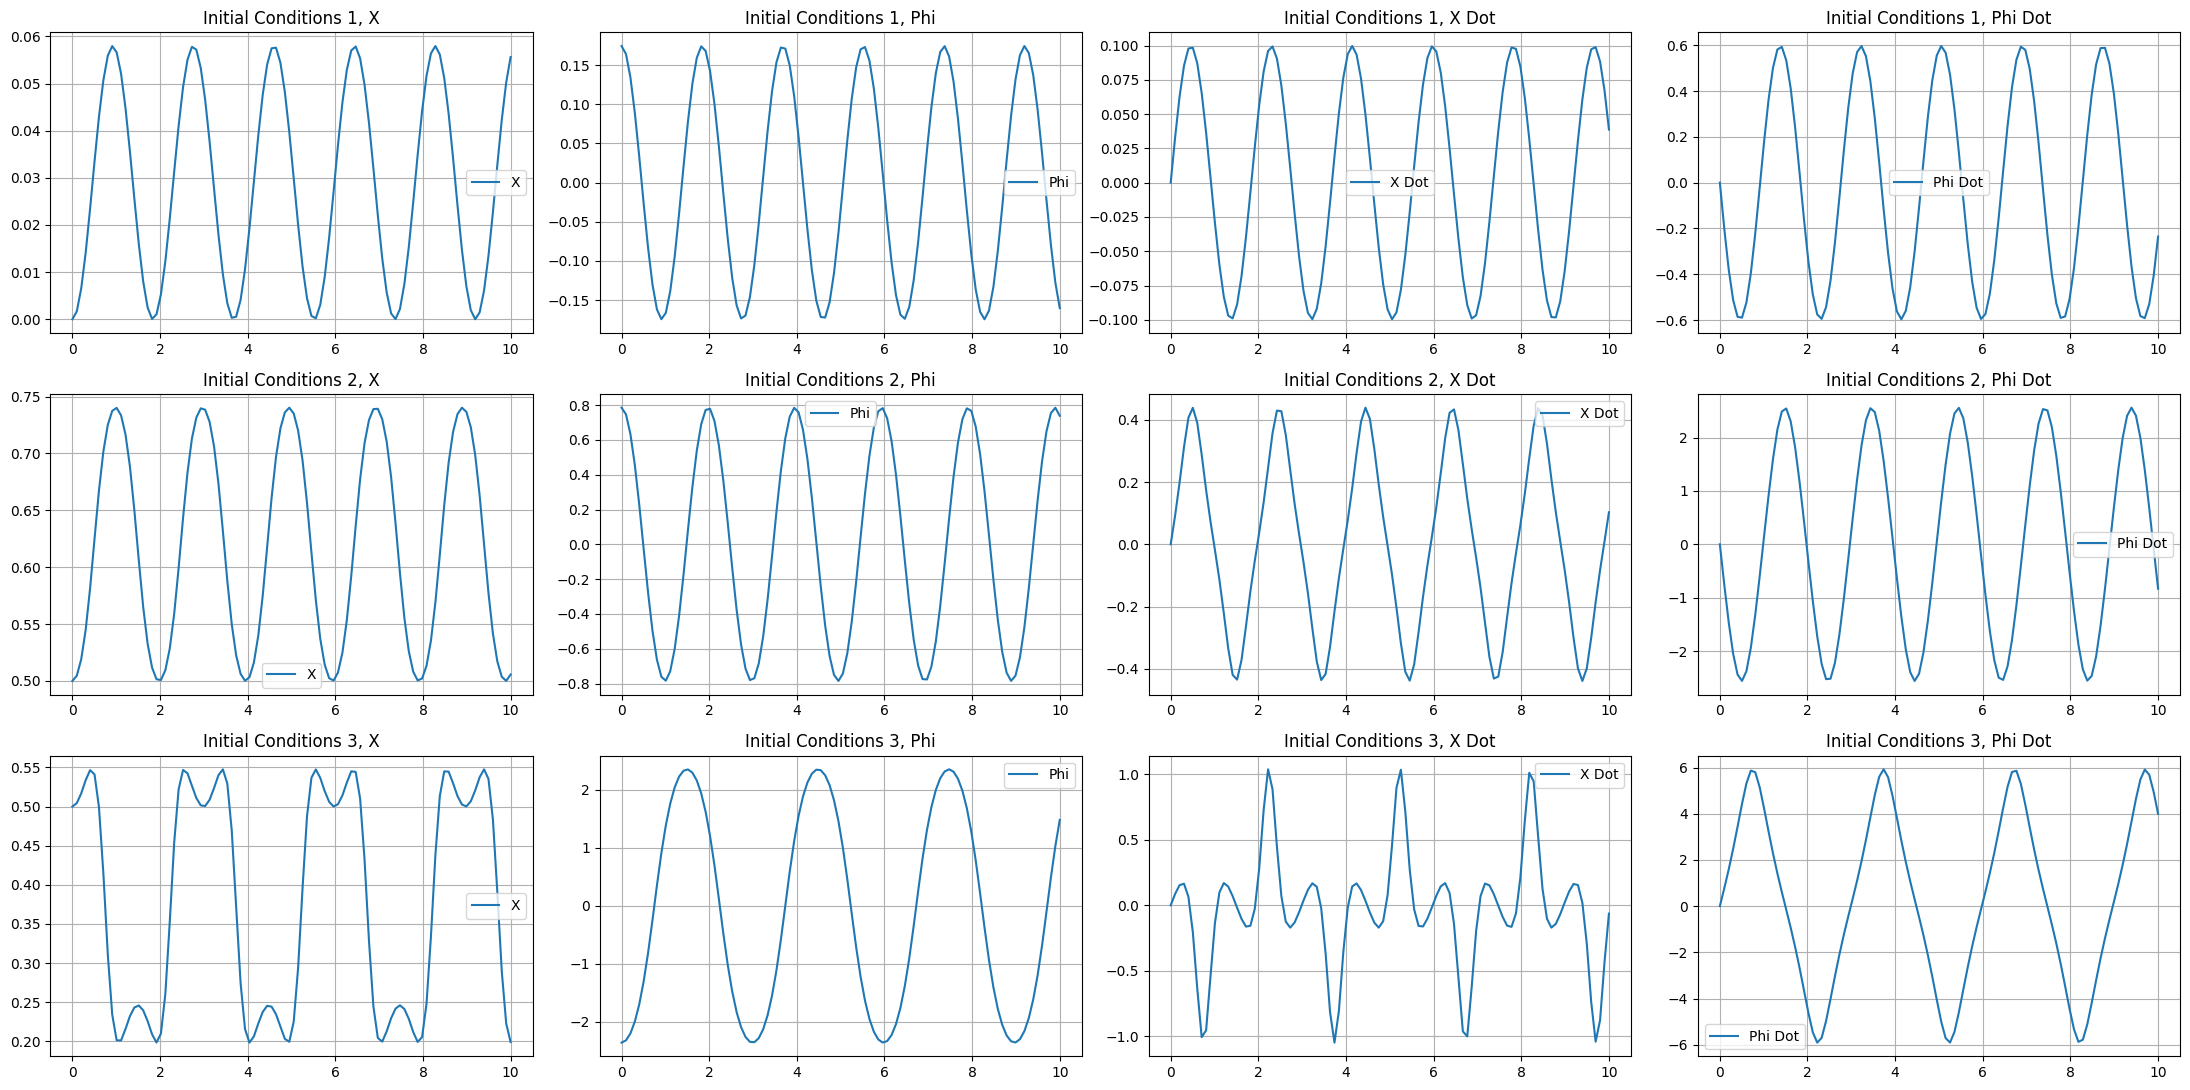
\includegraphics[scale=0.25]{plots/task2_plots.png}
\end{center}

\newpage

\subsection{Simulation}


\textbf{Initial condition 1: $\phi = 10^\circ$, $x = 0$}

\begin{figure}[htbp]
  \centering
  \begin{subfigure}[t]{0.45\linewidth}
    \centering
    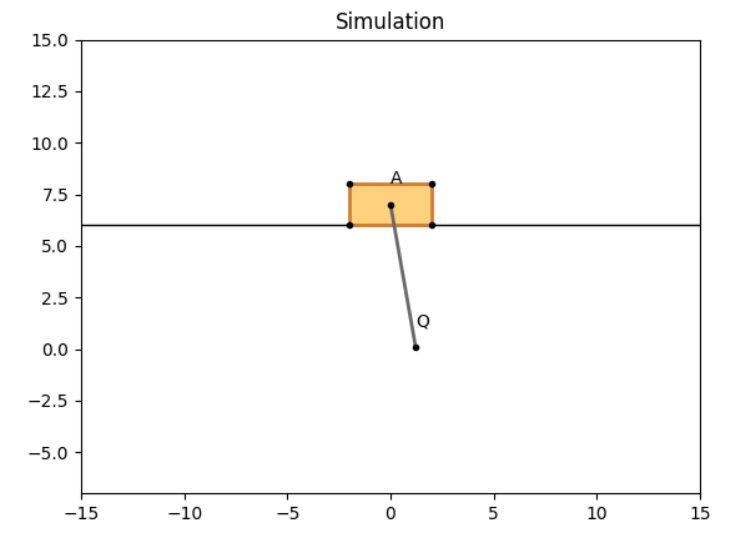
\includegraphics[width=\linewidth]{simulation/init1_1.png}
    \caption{}
  \end{subfigure}
  \begin{subfigure}[t]{0.45\linewidth}
    \centering
    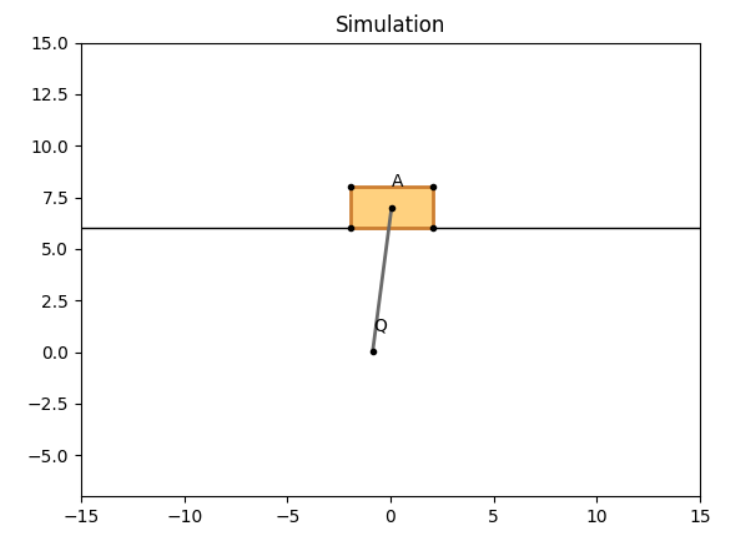
\includegraphics[width=\linewidth]{simulation/init1_2.png}
    \caption{}
  \end{subfigure}
\end{figure}

\textbf{Initial condition 2: $\phi = 45^\circ$, $x = 0.5$}

\begin{figure}[htbp]
  \centering
  \begin{subfigure}[t]{0.45\linewidth}
    \centering
    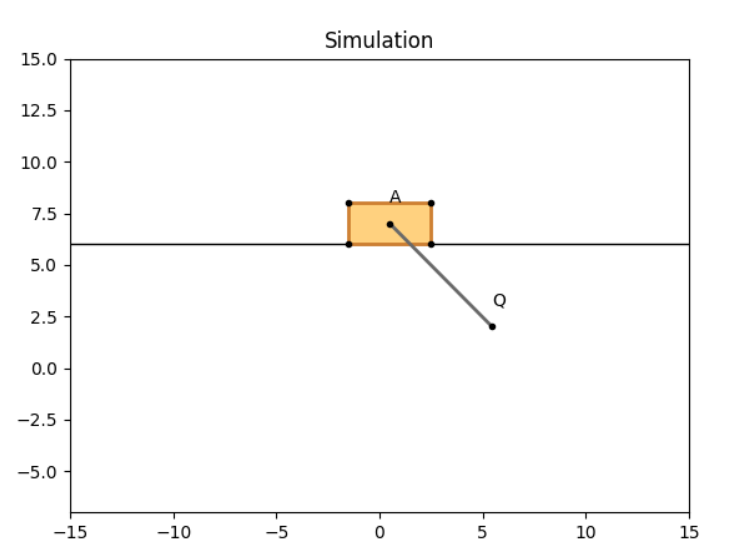
\includegraphics[width=\linewidth]{simulation/init2_1.png}
    \caption{}
  \end{subfigure}
  \begin{subfigure}[t]{0.45\linewidth}
    \centering
    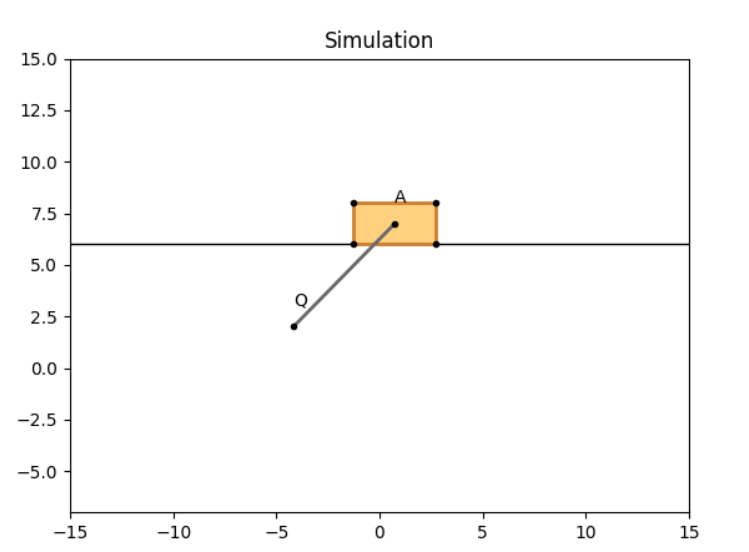
\includegraphics[width=\linewidth]{simulation/init2_2.png}
    \caption{}
  \end{subfigure}
\end{figure}

\newpage

\textbf{Initial condition 3: $\phi = -135^\circ$, $x = 0.5$}

\begin{figure}[htbp]
  \centering
  \begin{subfigure}[t]{0.45\linewidth}
    \centering
    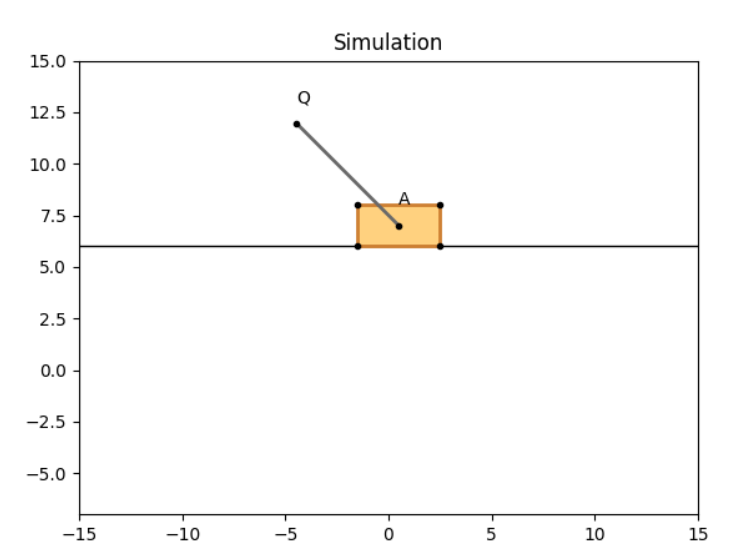
\includegraphics[width=\linewidth]{simulation/init3_1.png}
    \caption{}
  \end{subfigure}
  \begin{subfigure}[t]{0.45\linewidth}
    \centering
    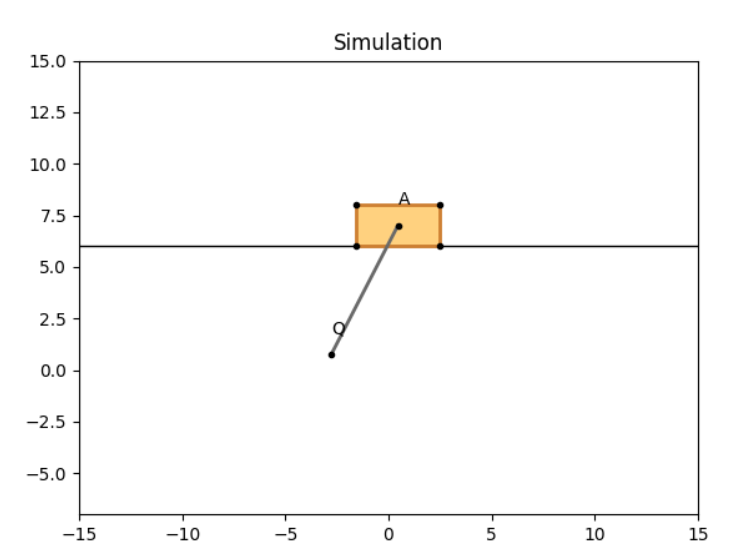
\includegraphics[width=\linewidth]{simulation/init3_2.png}
    \caption{}
  \end{subfigure}
  \begin{subfigure}[t]{0.45\linewidth}
    \centering
    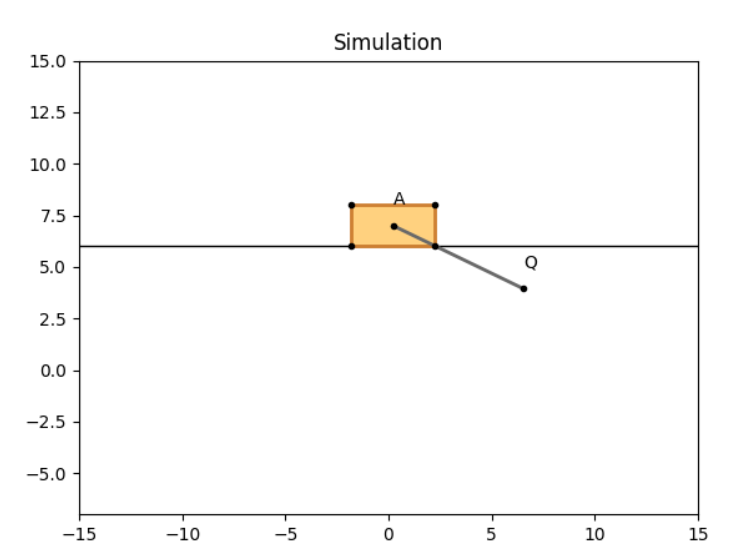
\includegraphics[width=\linewidth]{simulation/init3_3.png}
    \caption{}
  \end{subfigure}
  \begin{subfigure}[t]{0.45\linewidth}
    \centering
    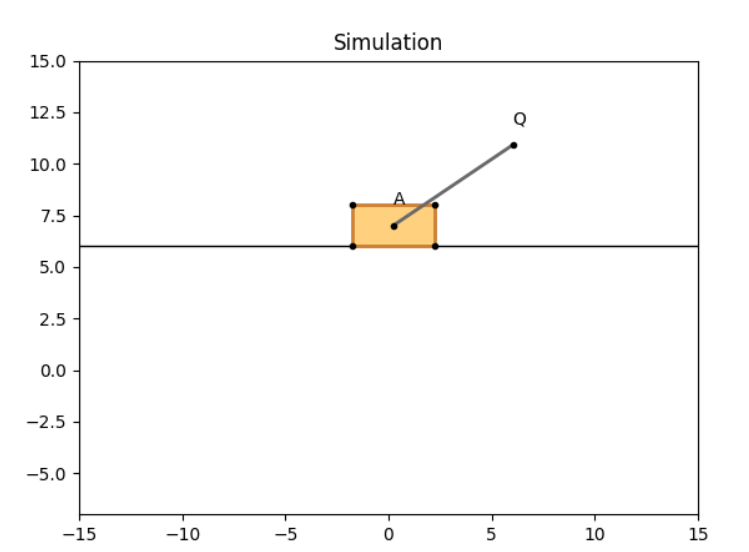
\includegraphics[width=\linewidth]{simulation/init3_4.png}
    \caption{}
  \end{subfigure}
\end{figure}

\section{Simulink}


\textbf{Initial condition 1: $\phi = 10^\circ$, $x = 0$}
\begin{figure}[htbp]
  \centering
  \begin{subfigure}[t]{0.4\linewidth}
    \centering
    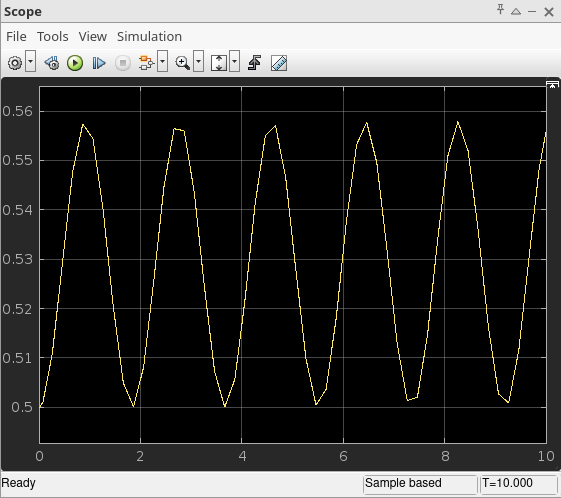
\includegraphics[width=\linewidth]{simulink/init1_x.png}
    \caption{x}
  \end{subfigure}
  \begin{subfigure}[t]{0.4\linewidth}
    \centering
    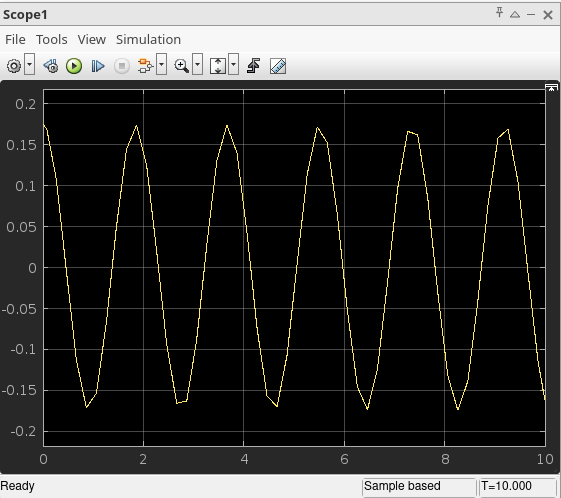
\includegraphics[width=\linewidth]{simulink/init1_phi.png}
    \caption{$\phi$}
  \end{subfigure}
\end{figure}

\newpage 


\textbf{Initial condition 2: $\phi = 45^\circ$, $x = 0.5$}
\begin{figure}[htbp]
  \centering
  \begin{subfigure}[t]{0.45\linewidth}
    \centering
    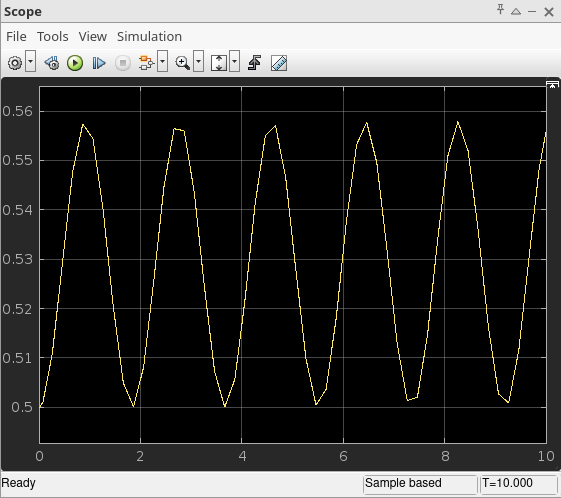
\includegraphics[width=\linewidth]{simulink/init1_x.png}
    \caption{x}
  \end{subfigure}
  \begin{subfigure}[t]{0.45\linewidth}
    \centering
    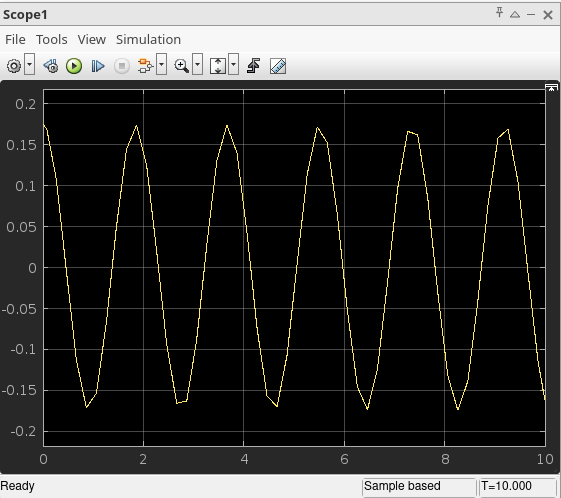
\includegraphics[width=\linewidth]{simulink/init1_phi.png}
    \caption{$\phi$}
  \end{subfigure}
\end{figure}

\textbf{Initial condition 3: $\phi = -135^\circ$, $x = 0.5$}

\begin{figure}[htbp]
  \centering
  \begin{subfigure}[t]{0.45\linewidth}
    \centering
    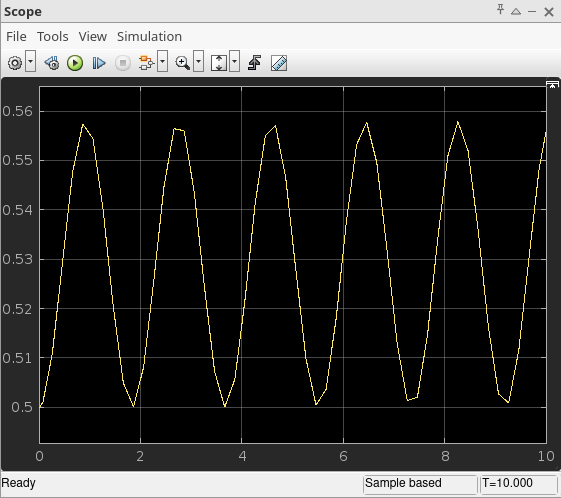
\includegraphics[width=\linewidth]{simulink/init1_x.png}
    \caption{x}
  \end{subfigure}
  \begin{subfigure}[t]{0.45\linewidth}
    \centering
    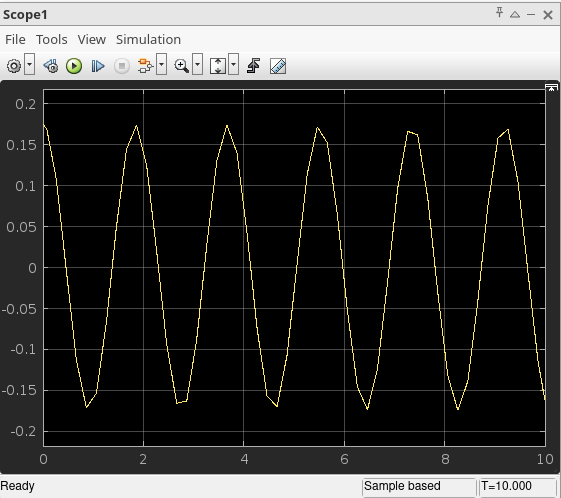
\includegraphics[width=\linewidth]{simulink/init1_phi.png}
    \caption{$\phi$}
  \end{subfigure}
\end{figure}

The plots approximately coincide with those obtained using the coding method.

\end{document}